\Chapter{Étude de plasmas magnétisés}
\chaptermark{Étude de plasmas magnétisés}
\begin{refsection}
Ce quatrième chapitre porte sur l'étude de deux cas concrets
chacun représentatif d'une configuration magnétique particulière : le filtre
magnétique avec le propulseur PEGASES et la colonne de plasma magnétisée de la
source d'ions négatifs CYBELE. 
A travers ces exemples, nous testons les possibilités du nouveau code MAGNIS,
tout en explorant la physique qu'il révèle. Les simulations sont discutées et
confrontées aux mesures expérimentales ainsi qu'aux résultats de modèles
statistiques.
En fin de chapitre, nous simulons une configuration typique de bord de tokamak,
de champ magnétique intense et où le transport est principalement de nature
turbulente. 
		 
\section{PEGASES, la barrière magnétique}
\subsection{Comparaison expérimentale}
\begin{figure}
  \centering
    \subfigure[]{\label{4-PegasesCarteDensiteBase}
    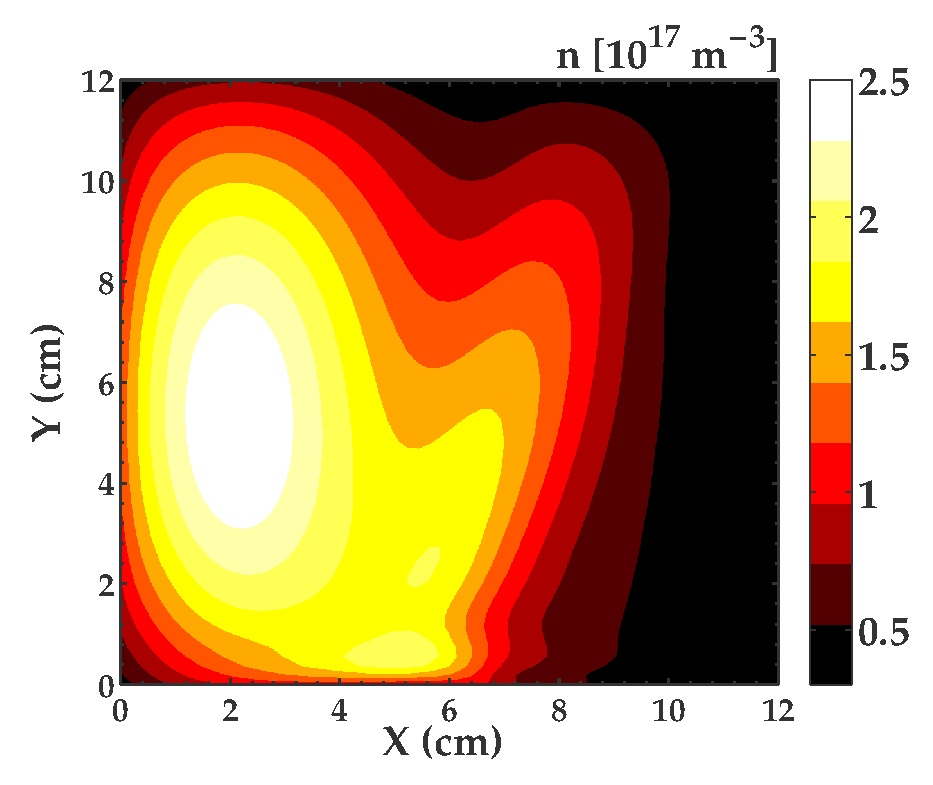
\includegraphics[height=4cm]{figures/4-PegasesCarteDensiteBase.eps}}
    \subfigure[]{\label{4-PegasesCartePotentielBase}
    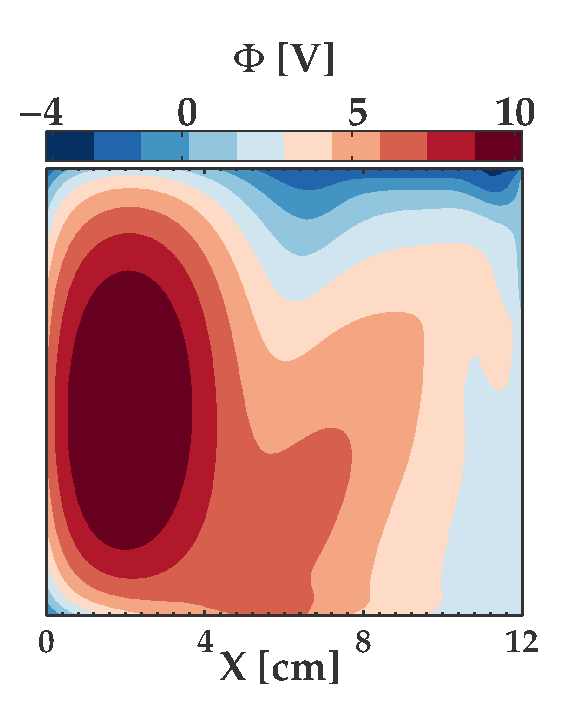
\includegraphics[height=4cm]{figures/4-PegasesCartePotentielBase.eps}}
    \subfigure[]{\label{4-PegasesCarteTemperatureBase}
    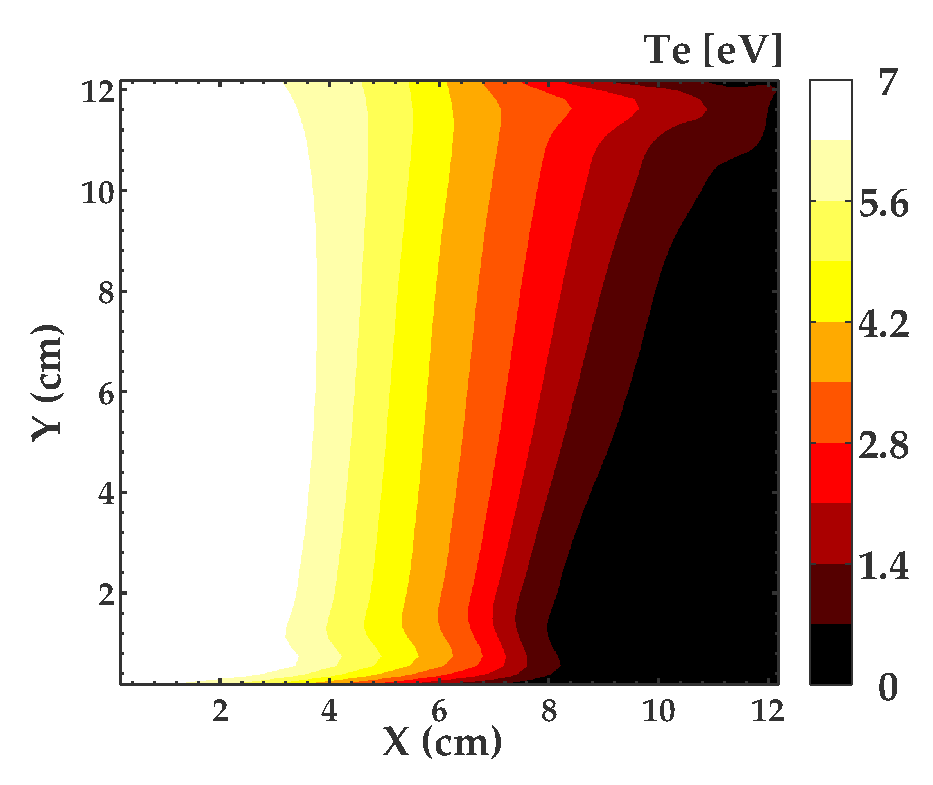
\includegraphics[height=4cm]{figures/4-PegasesCarteTemperatureBase.eps}}
    \caption{Cartes de densité\subref{4-PegasesCarteDensiteBase}~, de
    potentiel\subref{4-PegasesCartePotentielBase}~ et de
    température\subref{4-PegasesCarteTemperatureBase}}
    \label{pandas}
\end{figure}
\begin{figure}
  \centering
    \subfigure[]{\label{4-PegasesCarteVeBase}
    \includegraphics[height=4cm]{figures/4-PegasesCarteVeBase.eps}}
    \subfigure[]{\label{4-PegasesCarteViBase}
    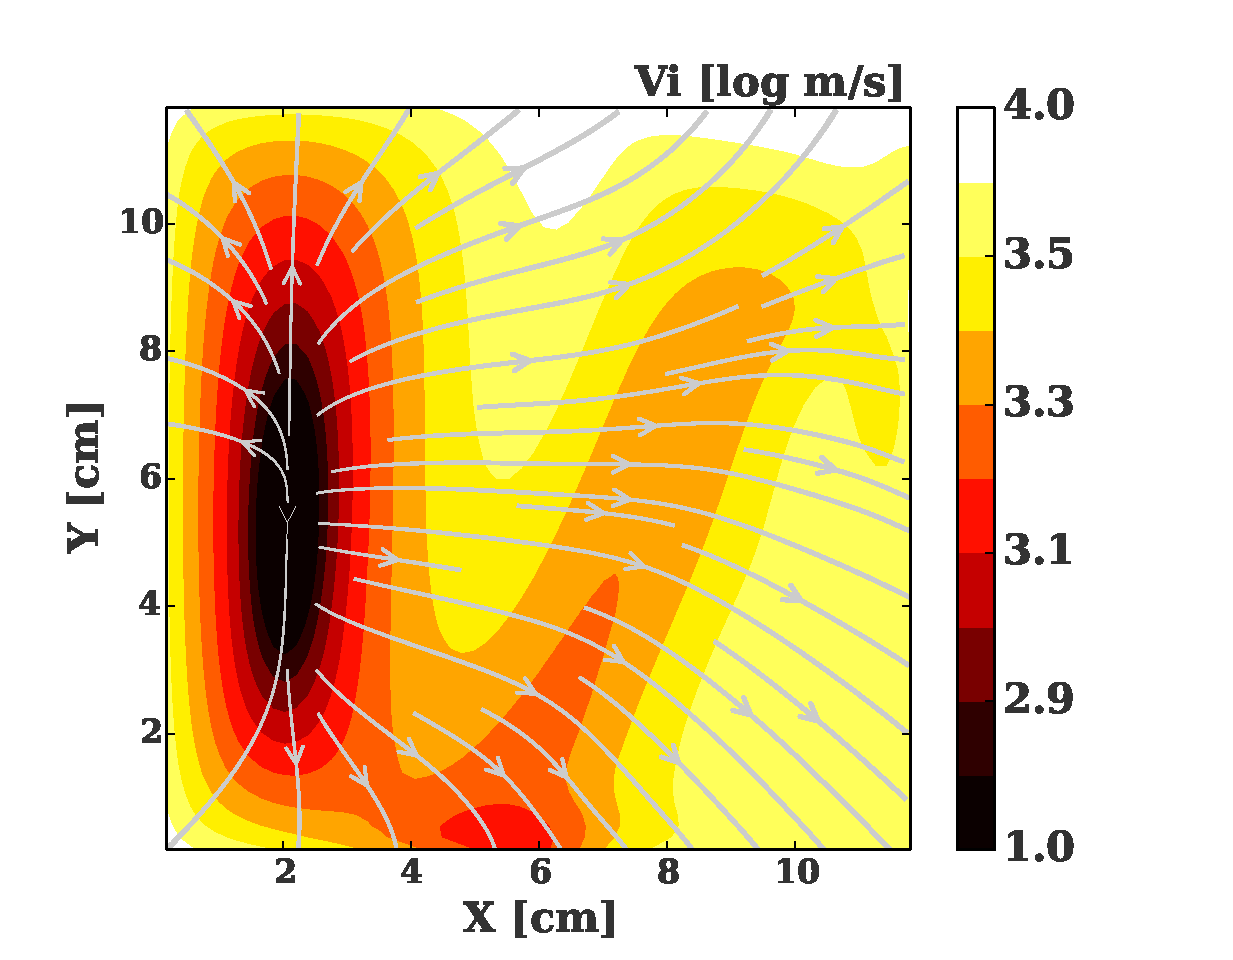
\includegraphics[height=4cm]{figures/4-PegasesCarteViBase.eps}}
    \caption{Cartes de densité\subref{4-PegasesCarteVeBase}~, de
    potentiel\subref{4-PegasesCarteViBase}~ et de
    température\subref{4-PegasesCarteTemperatureBase}}
    \label{pandas}
\end{figure}
			
	\subsubsection{Scan en pression}
	\subsubsection{Variations du champ magnétique}
\subsection{Transport du courant dans le cas de parois conductrices}
	\subsubsection{Influence du champ magnétique}
	\subsubsection{Transport à travers le filtre magnétique}
\subsection{Phénomènes intermittents, instabilités}
	\subsubsection{Vagues ioniques}
	\subsubsection{Instabilité "<finger">}
	
\section{CYBELE - Colonne de plasma magnétisée}
\subsection{Absence de courant extérieur}
	\subsubsection{Influence du champ magnétique}
	\subsubsection{Influence de la densité de gaz}
\subsection{Polarisation des parois}
		

\section{Plasma de bord de tokamaks}
%\bibliographystyle{apalike}
%\bibliography{biblio}
\end{refsection}
